
\begin{frame}{‌الگوریتم دایکسترا}
\begin{itemize}\itemr
\item[-]
الگوریتم دایکسترا مسئله کوتاهترین مسیر برای گراف وزن‌دار جهت‌دار
\m{G = (V,E)}
را وقتی وزن‌ها منفی نباشند حل می‌کند. به عبارت دیگر به ازای هر یال
\m{(u,v) \in E}
در الگوریتم دایکسترا لازم است داشته باشیم
\m{w(u,v) \geqslant 0} .
\item[-]
با یک پیاده‌سازی بهینه، الگوریتم دایکسترا می‌تواند در زمان کمتری نسبت به الگوریتم بلمن-فورد مسئله را حل کند.
\end{itemize}
\end{frame}


\begin{frame}{‌الگوریتم دایکسترا}
\begin{itemize}\itemr
\item[-]
الگوریتم دایکسترا به صورت زیر است.
\begin{algorithm}[H]\alglr
  \caption{Dijkstra} 
  \begin{algorithmic}[1]
  \Func{Dijkstra}{G, w, s}
   \State Initialize-Single-Source(G,s)
   \State S = $\emptyset$
   \State Q = $\emptyset$
   \For{each vertex u $\in$ G.V}
   		\State Insert(Q,u)
   	\EndFor
   	\While{Q $\neq \emptyset$}
   			\State u = Extract-Min(Q)
   			\State S = S $\cup$ \{u\}
   			\For{each vertex v in G.Adj[u]}
   					\State Relax(u,v,w)
   					\If{the call of Relax decreased v.d}
   							\State Decrease-Key(Q,v,v.d)
   					\EndIf
   			\EndFor
   	\EndWhile                       
  \end{algorithmic}
  \label{alg:merge}
\end{algorithm}
\end{itemize}
\end{frame}


\begin{frame}{‌الگوریتم دایکسترا}
\begin{itemize}\itemr
\item[-]
یک مثال از الگوریتم دایکستر در شکل زیر نشان داده شده است.
\begin{figure}
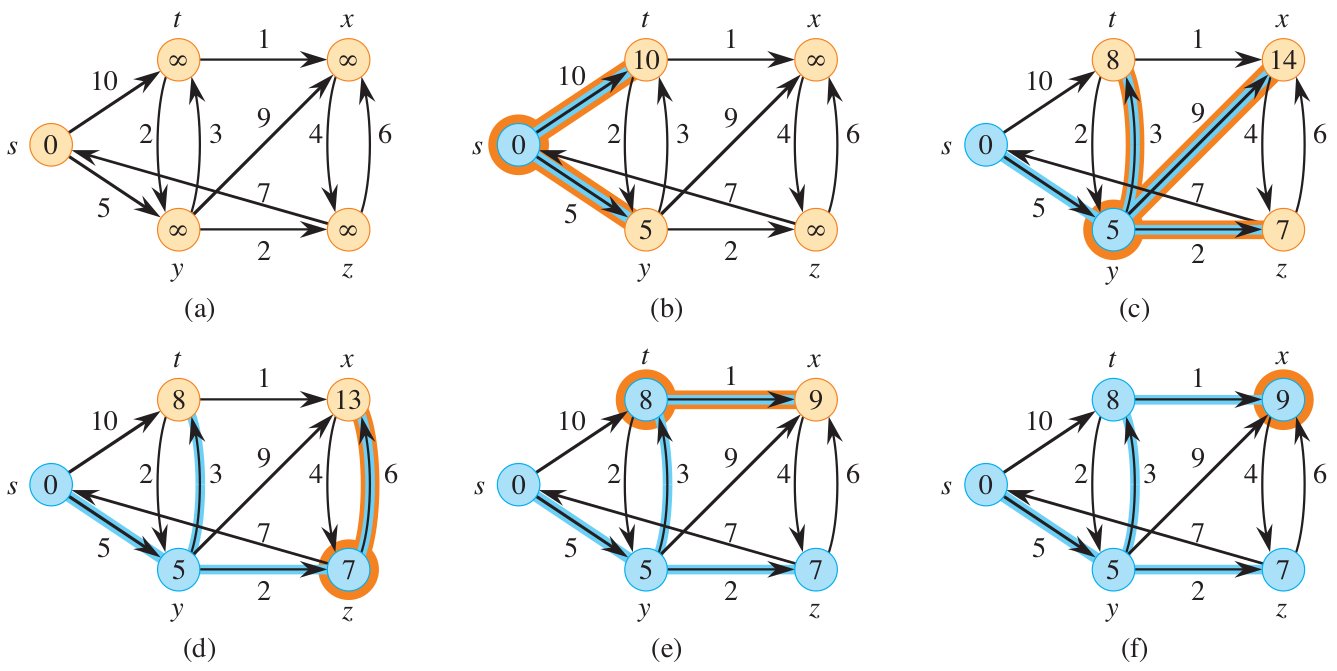
\includegraphics[width=0.9\textwidth]{figs/chap07/621-dijkstra}
\end{figure}
\end{itemize}
\end{frame}


\begin{frame}{‌الگوریتم دایکسترا}
\LR{
\begin{figure}[!ht]
 % \centering
  {\includestandalone[width=0.22\textwidth]{figs/chap07/d1}}
 {\includestandalone[width=0.22\textwidth]{figs/chap07/d2}}
 {\includestandalone[width=0.22\textwidth]{figs/chap07/d3}}
  {\includestandalone[width=0.22\textwidth]{figs/chap07/d4}}
  {\includestandalone[width=0.22\textwidth]{figs/chap07/d5}}
  {\includestandalone[width=0.22\textwidth]{figs/chap07/d6}}
 {\includestandalone[width=0.22\textwidth]{figs/chap07/d7}}
  {\includestandalone[width=0.22\textwidth]{figs/chap07/d8}}
  \iffalse
 \only<1>{\includestandalone{figs/chap07/d1}}
 \only<2>{\includestandalone{figs/chap07/d2}}
 \only<3>{\includestandalone{figs/chap07/d3}}
  \only<4>{\includestandalone{figs/chap07/d4}}
  \only<5>{\includestandalone{figs/chap07/d5}}
  \only<6>{\includestandalone{figs/chap07/d6}}
  \only<7>{\includestandalone{figs/chap07/d7}}
  \only<8>{\includestandalone{figs/chap07/d8}}
  \fi
  \label{fig:d1}
\end{figure}
}
\iffalse
\[
P =~\langle~c_1, \pause \pause c_2, \pause \pause c_3,\pause \pause 
c_4,  \pause c_5 ~\rangle
\]
\fi
\end{frame}



\begin{frame}{‌الگوریتم دایکسترا}
\begin{itemize}\itemr
\item[-]
مجموعهٔ 
\m{S}
شامل رئوسی است که کوتاهترین مسیر از مبدأ برای آنها تعیین شده است.
\item[-]
از آنجایی که الگوریتم دایکسترا همیشه نزدیک‌ترین رأس به مبدأ در
\m{V-S}
را به
\m{S}
اضافه می‌کند، این الگوریتم یک الگوریتم حریصانه است.
\end{itemize}
\end{frame}


\begin{frame}{‌الگوریتم دایکسترا}
\begin{itemize}\itemr
\item[-]
برای تحلیل زمان اجرای الگوریتم دایکسترا از تحلیل تجمعی استفاده می‌کنیم.
\item[-]
از آنجایی که هر رأس
\m{u \in V}
به مجموعهٔ
\m{S}
فقط یک‌بار اضافه می‌شود، هر یال در لیست مجاورت
\m{Adj[u]}
در حلقه
\code{for}
خطوط ۹ تا ۱۲ دقیقا یک‌بار در طول اجرای الگوریتم بررسی می‌شود.
بنابراین این حلقه در مجموع
به تعداد یال‌های گراف
تکرار می‌شود و
\code{Decrease-key}
در مجموع حداکثر
به تعداد یال‌ها
تکرار می‌شود.
هزینه بررسی همهٔ یال‌ها
\m{O(|E|)}
است.
\item[-]
حلقه
\code{while}
نیز به تعداد رئوس گراف تکرار می‌شود.
\item[-]
زمان اجرای الگوریتم دایکسترا به پیاده‌سازی صف اولویت بستگی پیدا می‌کند.
\item[-]
در یک پیاده‌سازی ساده صف اولویت توابع
\code{Insert}
و
\code{Decrease-key}
در زمان
\m{O(1)}
و تابع
\code{Extract-Min}
در زمان
\m{O(|V|)}
اجرا می‌شود.
\item[-]
بنابراین زمان اجرای الگوریتم
\m{O(|V|^2 + |E|) = O(|V|^2)}
است.
\end{itemize}
\end{frame}



\begin{frame}{‌الگوریتم دایکسترا}
\begin{itemize}\itemr
\item[-]
اگر صف اولویت با استفاده از هیپ پیاده‌سازی شود،
 توابع
\code{Extract-Min}
و
\code{Decrease-key}
در زمان
\m{O(lg|V|)}
اجرا می‌شوند.
\item[-]
بنابراین زمان اجرای الگوریتم
\m{O((|V|+|E|)lg|V|)}
خواهد بود.
\item[-]
در یک گراف همبند که تعداد یال‌ها بزرگتر یا مساوی تعداد رئوس است، الگوریتم دایکسترا در زمان
\m{O(|E| lg |V|)}
اجرا می‌شود.
\item[-]
یک پیاده‌سازی بهینه‌تر نیز با استفاده از هرم فیبوناچی برای الگوریتم دایکسترا وجود دارد که زمان اجرا را به
\m{O(|E| + |V| lg |V|)}
کاهش می‌دهد که در اینجا به آن نمی‌پردازیم.
\end{itemize}
\end{frame}